\documentclass[sigconf,authorversion,nonacm]{acmart}

\settopmatter{printacmref=false}
\usepackage{xcolor}
\usepackage{graphicx}


%%
%% \BibTeX command to typeset BibTeX logo in the docs
\AtBeginDocument{%
  \providecommand\BibTeX{{%
    Bib\TeX}}}

\begin{document}

\title{CSCI-582 Project Report: "Inference Performance Study on Oak-D Camera"}

\author{Cameron Legg}
\affiliation{%
 \institution{Colorado School of Mines}
 \city{Golden}
 \state{CO}
 \country{USA}
 }

\author{Ben Hempelmann}
\affiliation{%
 \institution{Colorado School of Mines}
 \city{Golden}
 \state{CO}
 \country{USA}
}

\maketitle

\section{Introduction}
In this project, we did a study with the Oak-D camera, operating on the Nvidia Orin NX. We vary parameters such as the number of shaves (cores), inference threads, and video size while benchmarking FPS and power consumption. We also run the same benchmark on the CPU and GPU of the Orin NX for extra comparison. Lastly, we discuss what we believe is the optimal number of shaves and inference threads for our model on the Oak-D camera. We run the benchmarks while inferencing human falls with a YOLO model on a 5 minute video.

\section{Targeted domain {\small [2 pts]}}
% Explain the application or the domain you have presented on and experimented with. 

The application that we chose to target for this paper is YOLO (You Only Look Once), a computer vision platform that is used for real-time object detection and tracking using bounding boxes. The upside to using this framework is that it is easily compiled and trained, and can be lightweight depending on if it needs to be deployed on an edge-computing device. The specific use case that we chose to use YOLO for is human fall detection, specifically with real time monitoring for at risk individuals.

Current methods for fall detection are intrusive meaning that a physical device is required to be worn by the person being monitored. Worn devices almost always need to be battery-powered and can be easily forgotten whereas image based classification can be set up in a desired location and forgotten about. The overall motivation of this project is to benchmark performance of YOLO models and determine if it is feasible to deploy them in edge-environments.


\section{Motivation: The need for acceleration {\small {[2 pts]}}}

Detecting human falls may require edge devices to be placed around in many different places. These places could have power restrictions or size restrictions. It is not very practical to place a computer, running a full size graphics card everywhere a camera is needed. In this case, an accelerator is perfect because inferencing can be done rather quickly with a device that is smaller and consumes low power. This is due to the accelerator being designed for that specific application.

\section{Related work {\small {[8 pts]}}}
% Starting with the short summary of the paper you presented, explain how other work tackled the acceleration problem for the targeted domain. For the paper you presented, state the key idea(s), solution(s) and contribution(s) of the paper(s) and briefly talk about the technical details of their approach.

% You don't need to read additional papers, however, in your summary above, please cite at least 3 other related works that you learned about while you are reading the paper you presented. 


The paper we read was \textit{Human Fall Detection using YOLO: A Real{-}Time and AI{-}on{-}the{-}Edge Perspective} by Ali Raza et al. [1] focused on detecting falls in a non-intrusive way. The authors defined intrustive as using wearables on on-body sensors. Their idea was to detect human falls using computer vision on an edge device. How they attacked this problem was by running a YOLO Darknet model trained for detecting human falls on a Raspberry Pi with the Oak-D camera and its computer vision accelerator. The Oak-D camera that they used is the same camera that we used in our project. This paper contributes to the scientific community a way to run YOLO models on the Oak-D camera by converting the PyTorch files to OpenVino formatting. The strengths of the paper include proving that there is an effective, non-intrusive way to detect human falls using a computer vision approach. They also proved that fall detection can be done on an edge device, which could theoretically be placed anywhere. The main weakness of this paper was that they did not compare power consumption, which is an aspect that we decided to dive into in our project.

Some other approaches to inferencing on edge devices included using other accelerators than the Oak-D camera. One approach by S. Sam et al. uses the Coral Edge TPU as an accelerator to run a YOLO model to detect traffic lights. R. A. Amin et al. also do YOLO inferencing, but using an FPGA. Another source related to this paper is Rey L. et al. [4] researching running AI models on Nvidia Jetson devices for use in UAVs and drones.

All of these related work involve running computer vision and AI applications on some sort of edge device, with the goals in mind to keep smaller form factors and have reduced power consumption as compared to inferencing on full-size GPUs. Each of these contribute some information on how to efficiently run inferencing on smaller devices using YOLO models on different accelerators and hardware.

\subsection{Current Limitations}
% Briefly talk about weaknesses of current approaches, if available. 

Considering that YOLO stands for You Only Look Once, there are some obvious limitations of the technology when it comes to tracking individuals for fall detection. The first and most notable limitation is the lack of information transfer between frames. The way that YOLO is able to detect if a fall has taken place is by examining the bounding box (and its shape) of a person in frame and determining if the shape of that bounding box is consistent with the training data that it was given. Since YOLO doesn’t retain memory between images, it can’t tell if a person is just laying down or in an awkward position or if they transitioned from a standing position to a fall. More complex models that can track across frames would be needed to detect falls. 

Another weakness of the current approach is the need for a person to be in frame of the camera at all times to detect if they have fallen which might require many cameras depending on if a person wants full coverage of an area or house. This could be expensive in comparison to wearable options.


\section{Project Description  {\small {[2 pts]}}}

\subsection{Benchmark}
Our benchmark ran the YOLO model inferencing of the 5 minute video consisting of human falls on the CPU, GPU, and Oak-D camera's accelerator. During the inferencing process, the benchmarking Python script records the average power consumption and FPS over the previous 300 frames. We ran the benchmark many times, altering the number of shaves (cores) and inference threads to be used on the camera's hardware.

\subsection{Accelerated Kernels}
Inferencing with a YOLO model is a highy parallelizable task. This is because many kernels of the inferencing process are parallelizable. For example, a kernel that can be accelerated is the convolution process. Other kernals, such as activation functions can also be parallelized, making this application perfect for parallelization and acceleration. The Orin NX can take advantage of cuda kernals to speed of neural processing and matrix operations while the Oak-D camera can take advantage of both it Nerual Computer Engine and the Shave cores to improve performance for parallel applications.

\subsection{Targeted Platforms}
We ran the YOLO inferencing benchmark on the following platforms:
\begin{itemize}
    \item \textbf{Nvidia Orin NX GPU} \\ 1024 CUDA Cores
    \item \textbf{Nvidia Orin NX CPU} \\ Arm Cortex A78AE 8-core CPU
    \item \textbf{Oak-D Camera} \\ This camera consists of a system on a chip architecture, running the Intel Movidius Myriad X Vision Processing unit. This accelerator has 2 Leon CPU cores. It also has 16 SHAVE cores - SHAVE cores is company's terminology for vector processing units. This device also has a max power consumption of 4.5W. Lastly, the device has 2 neural compute engines built into the chip.
\end{itemize}

\subsection{Challenges}
% What are the challenges you have faced while using this interface and how you tackled them?
% Maybe talk about how we origionally started with the raspberry pi, but couldn't due to need to measure power consumption. Talk about the conversion process. Think of other challenges.

Over the course of this project, we encountered several challenges that changed the course of the project and forced us to deviate from our original plan. What we had originally planned to do was use a Raspberry Pi as our main platform and hook the Oak-D camera up to it via USB. The main reason for this is that we wanted to mimic a real-world scenario where an application like this might be deployed. Raspberry Pi boards are inexpensive and deployed as edge computing devices quite commonly and replicating this would allow us to mimic a real environment. The problem that we ran into was that there isn’t a very reliable way to measure power draw without external adaptors and even then, measuring USB power can be difficult. What we ended up doing to solve this issue was switching from a Raspberry Pi to the Nvidia Orin NX. This platform has built in support for measuring power draw via software which was extremely useful to us. 

Another challenge that we ran into was converting our YOLO models into a compatible format for the Oak-D camera (OpenVino), and compiling models for different video qualities. One major testing point that we wanted to examine was the impact of different shave counts on Oak-D performance. The issue is that each model has to be explicitly compiled to use a set number of shaves and cannot be varied at runtime. The only solution to this problem is to compile a new model for every shave count that you want to test resulting in a lot of data. In order to test the performance of a YOLO model on different video qualities you need to completely retrain the PyTorch version of the model from scratch which takes a significant amount of time. On top of that, the model needs to be converted to OpenVino format for every shave count once again.




\section{Experiment Setup  {\small {[2 pts]}}}

\subsection{Methodology}  

\begin{itemize}
    \item \textbf{Training YOLO} \\ Training the YOLO model was the first step of the process. We found an already-labeled human fall dataset on Kaggle which consisted of 374 images for training and 111 for validation. Each of these images were labeled with Walking, Sitting, and Fall Detected. Essentially, if someone is seen laying down, Fall Detected is triggered. We then used this dataset to train a YOLO v11 model using the T4 GPU in Google Colab.
    \item \textbf{Converting the YOLO PyTorch File} \\ To run the YOLO model on the Oak-D camera, we needed to convert the PyTorch weights file to OpenVino format. The most reliable way to do this conversion was by using the online tool at https://tools.luxonis.com/. This site allows you to upload the PyTorch model and select the number of SHAVEs it should be compiled for. Afterwards, you can download the correctly formatted files and run them directly on the Oak-D camera. 
    \item \textbf{Runtime Framework / Programming Interfaces} \\ - To run the inferencing on the Oak-D camera, we used the Depth AI Python Library, which is a library designed for running inferencing on the Intel Myriad Vector Processor. This library is capable of running the YOLO model after it has been converted to OpenVino format. \\ - To run the inferencing on the CPU and GPU, we used the Ultralytics Python library, which utilizes CUDA when inferencing is done on the Nvidia GPU and OpenMP when inferencing is done on the CPU.
    \item \textbf{Benchmark} \\ The benchmark was written using Python. The script changes the number of SHAVES, and inference threads used while inferencing with YOLO on a 5-minute video. We collected benchmarks for SHAVE numbers 1, 2, 4, 8, 10, 12, 14, and 16 while altering the inference thread numbers 1, 2, 3. We also ran the benchmark on the CPU and GPU. This means that we ran 26 different benchmarks, collecting the average power consumption and frame rate every 300 frames for each benchmark. The benchmark saved these datapoints out to CSV files for each hardware device or shave + thread combination. Because of the way we collected the data (averages every 300 frames), every CSV had the same number of data points, allowing for easier future comparison.
\end{itemize}

\subsection{Metrics measured and Comparisons made}
% What are the metrics (e.g. time, power, energy, etc.) being measured? What is being compared (e.g., applications and/or HW)? Through which methodology? What is your baseline?
% CPU GPU Oak-D shaves threads
There are several metrics that we decided to measure for this project, mainly FPS and power draw. Since the application of this project is intended to be deployed to an edge device/system, we figured these were the most important metrics to measure. For testing, we streamed a 5 minute video containing falls to both the Oak-D camera and the Orin NX GPU and ran the YOLO models as if they were processing a live video. This allowed us to get consistent results across devices while maintaining the same input. Since power draw can fluctuate quite a bit on any system, average power draw was used to eliminate outlier samples. Given these metrics, we decided to test the performance of the Oak-D camera vs. the performance of the Orin NX (both cpu and gpu) and determine which has the best power draw to FPS ratio. We also decided to measure the impact of shave counts on the performance of the Oak-D running YOLO on its own.


\section{Results {\small {[9 pts]}}}  
% Present your results (with charts) here. For each experiment you did:
% \begin{itemize}
%     \item Insert a chart/figure/table 
%     \item Explain the information that chart/figure/table gives
%     \item Interprete results. Refer to more data, if available, to support your interpretation. 
%     \item Try to just cover what we talked about in the presentation. Add a little more data on the smaller video file size (352 x 240)
% \end{itemize}

% There is no min/max limit on the charts. Try to logically group the information if you could. For example, you may include one chart for time measurement, another for power/energy, and another for the breakdown of the performance (data movement overhead, etc.). I expect this to be the most detailed section of your report.

% Also, please address the feedback I have given during your project presention.

\begin{itemize}
    \item \textbf{Power consumption VS FPS} \\ For this comparison, we created a scatterplot, comparing the average power consumption over the entire video vs the average FPS over the entire video. 
    \begin{figure}[h] % [h] = here
        \centering
        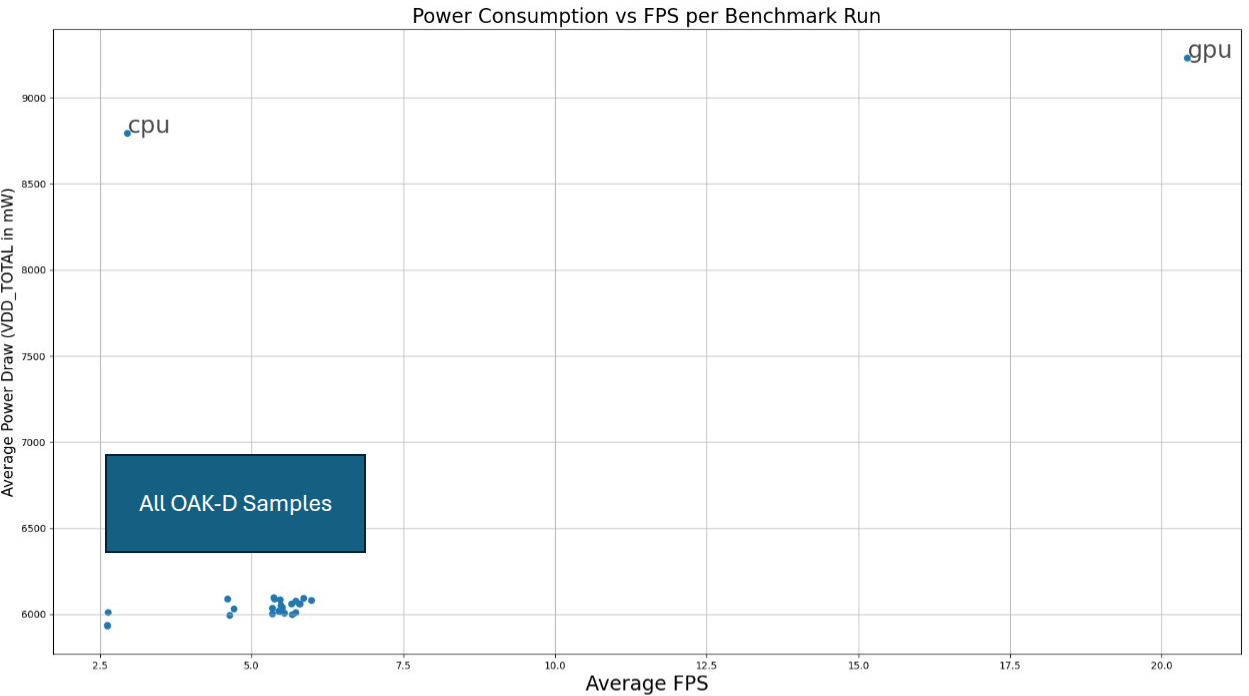
\includegraphics[width=0.5\textwidth]{figures/scatter1.png}
        \caption{Power consumption VS Frame Rate}
        \label{fig:your_label}
    \end{figure}
    \\ In Figure 1, you can see that the GPU consumed lots of power and had a high frame rate. The CPU consumed lots of power, but had a low frame rate. Also, it is visible that the Oak-D samples consumed much less power than the CPU and GPU, and had better frame rates than the CPU.
    \begin{figure}[h] % [h] = here
        \centering
        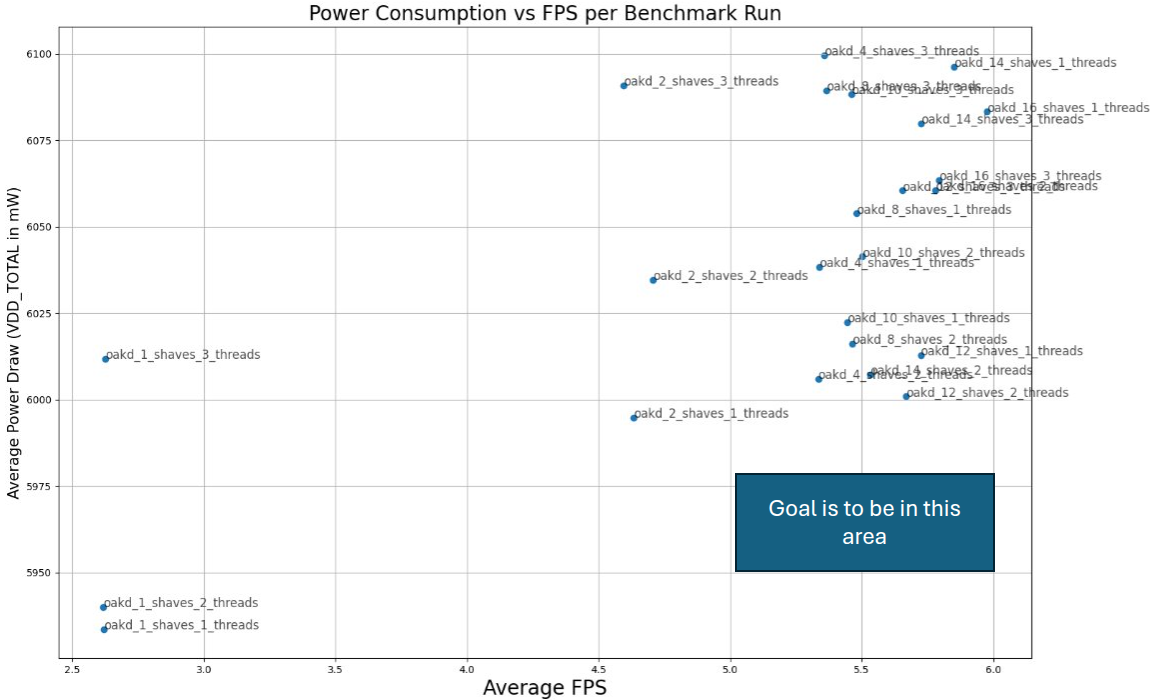
\includegraphics[width=0.5\textwidth]{figures/scatter2.png}
        \caption{Zoomed In - Power consumption VS Frame Rate}
        \label{fig:your_label}
    \end{figure}
    \\ In Figure 2, it is evident that setting the number of SHAVES to 1 resulted in the worst performace, but also lowest power consumption. In general, increasing the number of SHAVES yields a higher performance, but also higher power consumption. For the application of human fall detection on an edge device, an optimal amount of SHAVES and inference threads that yields in high FPS, but low power consumption is ideal. From this scatterplot, we bleieve that running the Oak-D camera with 12 shaves and 2 inference threads results in an optimal power comsumption to FPS ratio.
    
    \item \textbf{Frame vs FPS} \\ For this comparison, we compare the frame number, and the average FPS over the last 300 frames while varying the number of SHAVES, keeping the number of inference threads constant.
    \begin{figure}[h] % [h] = here
        \centering
        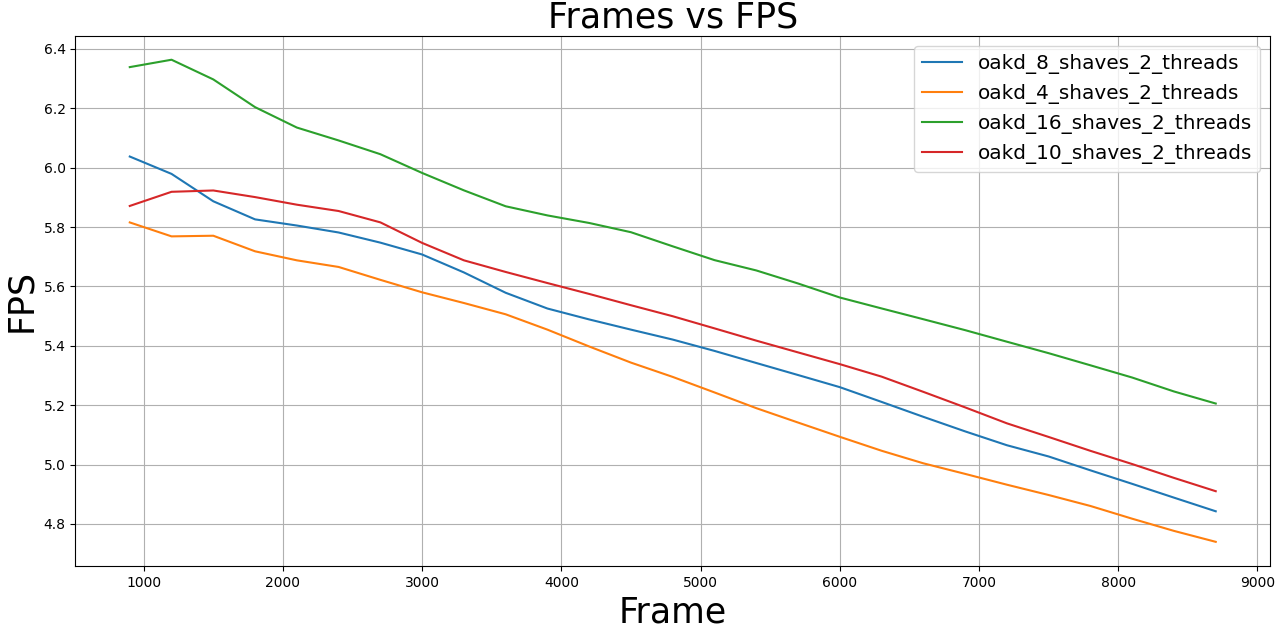
\includegraphics[width=0.5\textwidth]{figures/shavesvfps.png}
        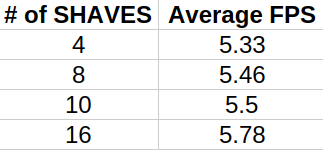
\includegraphics[width=0.2\textwidth]{figures/shavesvfpstable.png}
        \caption{Frame vs FPS}
        \label{fig:your_label}
    \end{figure}
    \\ In Figure 3, the 16 SHAVES model has the highest average FPS at 5.78 FPS, while the 4 SHAVES model has the lowest average FPS at 5.33 FPS. Given this figure, it is evident that increasing the number of SHAVES results in a higher frame rate.

    \clearpage
    \item \textbf{Frame vs Power Draw} \\For this comparison we measured the average power draw for different models over the course of the video being streamed to the YOLO models.
    \begin{figure}[h] % [h] = here
        \centering
        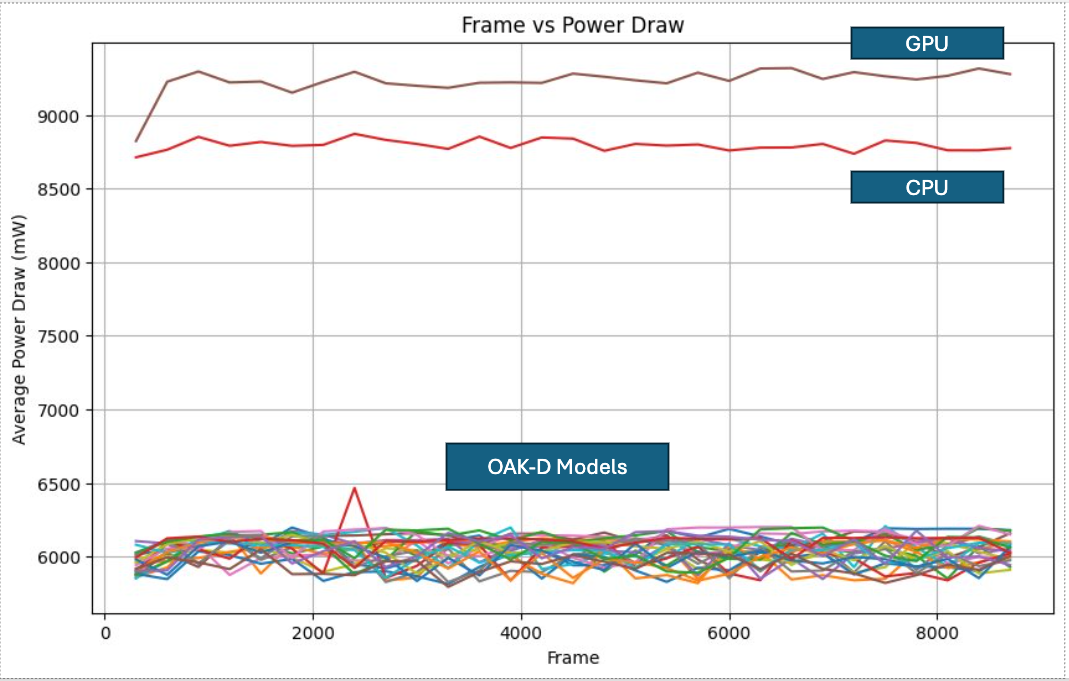
\includegraphics[width=0.5\textwidth]{figures/fram-vs-powerdraw-scatter.png}
        \caption{Frame vs Power Draw}
        \label{fig:your_label}
    \end{figure}
    
    Figure 3 serves merely to highlight the difference in power draw between the Orin NX CPU, GPU, and the Oak-D camera. The Oak-D processor has a max power draw of around 5w and running the models the way that we did maxed out the power draw.

    \item \textbf{Power Draw for Different Shave Counts} \\ This comparison helps distinguish how the power draw of Oak-D camera varries based on the shave count
    
    \begin{figure}[h] % [h] = here
        \centering
        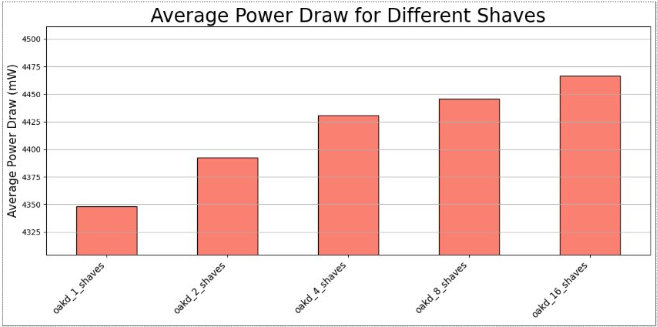
\includegraphics[width=0.5\textwidth]{figures/power-draw-shave.png}
        \caption{Power Draw for Different Shave Counts}
        \label{fig:your_label}
    \end{figure}

    This figure clearly highlights how increasing the number of shave cores used during processing increases the power draw of the Oak-D camera. One interesting point to note is that due to the various number of processors, power draw can be maxed out even with a smaller number of cores, especially when the number of cores is only slighlty varried. Some interesting furture work would be to test a lighter workload and isolate the different processors on the Oak-D camera, measuring the power draw in the process.

    \item \textbf{Varying Thread Count for the Same Shave} \\Another aspect of the Oak-D models that can be tuned is the (software) thread count. These threads can take advantage of most of the processors on the Oak-D chip and allow for some level of parallelism to be achieved.
    \begin{figure}[h] % [h] = here
        \centering
        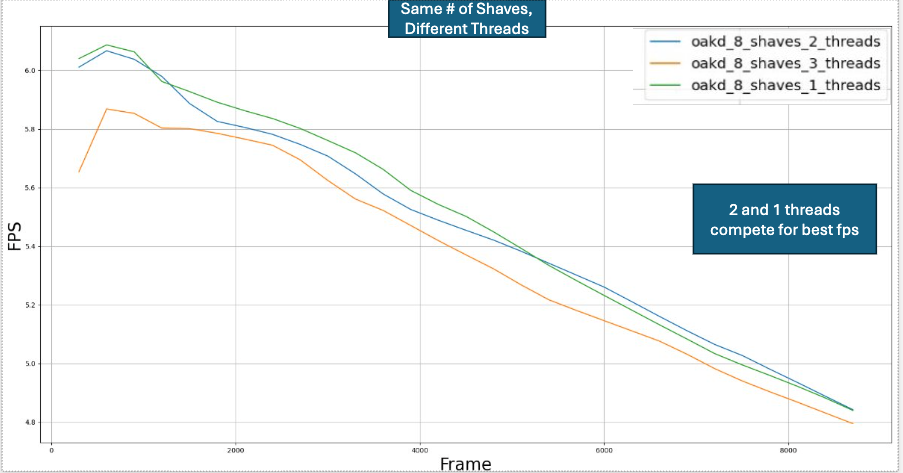
\includegraphics[width=0.5\textwidth]{figures/same-shave-thread-8.png}
        \caption{FPS vs Thread Count for 8 Shaves}
        \label{fig:your_label}
    \end{figure}
    \begin{figure}[h] % [h] = here
        \centering
        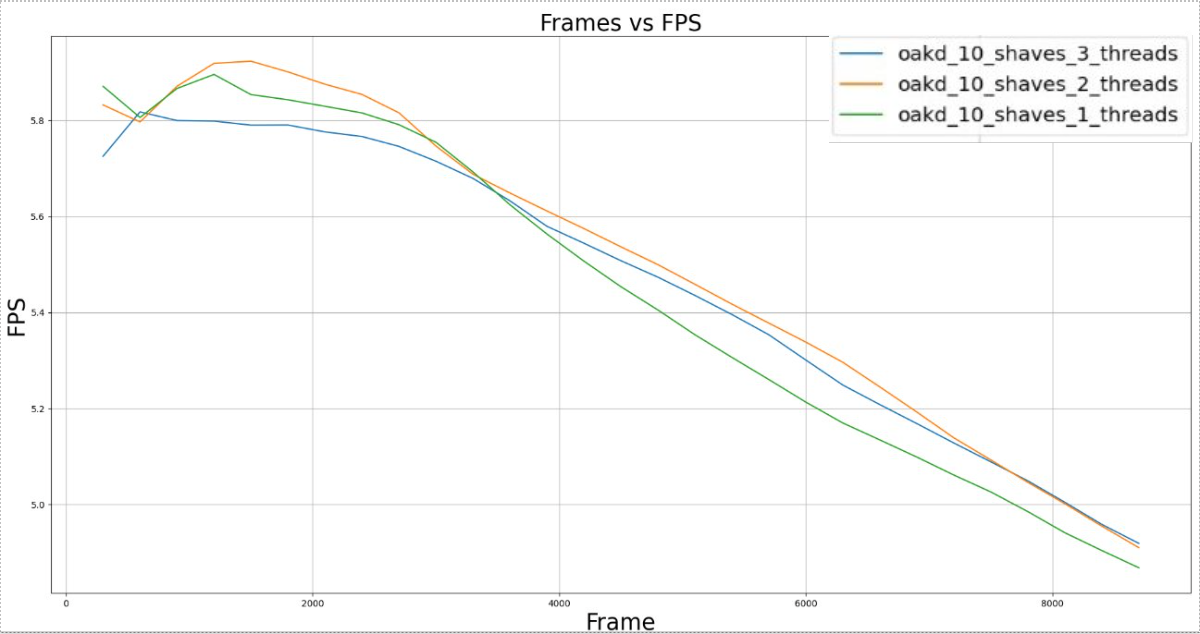
\includegraphics[width=0.5\textwidth]{figures/same-shave-thread-10.png}
        \caption{FPS vs Thread Count for 10 Shaves}
        \label{fig:your_label}
    \end{figure}

    Figures 6 and 7 highlight the performance of the YOLO models running on the same shave count but different thread counts. The maximum number of threads that can be set for this system is 3, but despite the potential for parallelism, we didn’t observe any trend in FPS for the different thread counts. The most plausible explanation for this lack of speedup is due to the application that is being run. YOLO processes a single image at a time and once that image is finished processing, it moves on to the next image. Since it isn’t processing multiple images at once, parallelism at the image level isn’t really possible. Other applications might be able to take advantage of these thread counts and it would be interesting to see if there is much performance to be gained in using them.
    

    \item \textbf{Changing Input Video Resolution} \\
    The original 5 minute video we ran for all of the previous benchmarks was 720x480 resolution. Before performing this experiment, we had assumed that decreasing the input video resolution would increase performance, however, we came to the conclusion that it does not. We downsized the same video to 352x240 and ran the same benchmark with that, but the frame rate and power consumption was extremely similar to the previous benchmarks. For example, the Oak-D benchmark with 10 shaves and 2 threads with the smaller video size had an average FPS of 5.81, while the same model on the large video resolution had an FPS of 5.5. This difference is too insignificant to conclude that FPS actually increased.\\ After looking into this issue, we learned that the YOLO models actually scale the resolution up / down to the training photo size before doing inferencing, which was we trained on 640p.
\end{itemize}

\section{Link to Source and other resources {\small {[3 pts]}}} 

\begin{itemize}
    \item \textbf{Benchmark Source (made by us) and Results} - \href{https://github.com/cameron-legg/BenchmarkingYOLOOakD}{https://github.com/cameron-legg/BenchmarkingYOLOOakD}
    \item \textbf{Final Presentation} - \href{https://github.com/cameron-legg/BenchmarkingYOLOOakD/blob/main/FinalPresentaiton.pdf}{https://github.com/cameron-legg/BenchmarkingYOLOOakD/blob/main/FinalPresentaiton.pdf}
    \item \textbf{Fall Detection Dataset} - \href{https://www.kaggle.com/datasets/uttejkumarkandagatla/fall-detection-dataset?resource=download}{https://www.kaggle.com/datasets/uttejkumarkandagatla/fall-detection-dataset?resource=download}
    \item \textbf{PyTorch to OpenVino Conversion} - \href{https://tools.luxonis.com/}{https://tools.luxonis.com/}
    \item \textbf{Oak-D Setup} - \href{https://docs.luxonis.com/software/depthai/manual-install/}{https://docs.luxonis.com/software/depthai/manual-install/}
    \item \textbf{A Tutorial We Looked At} - \href{https://learnopencv.com/object-detection-on-edge-device/}{https://learnopencv.com/object-detection-on-edge-device/}
\end{itemize}

\section{Project/class Takeaway {\small {[2 pts]}}}  
% Write a brief paragraph on what you have learned ``new" regarding performance analysis and overall on ``compute acceleration". Please also include your honest, brief opinion on how this new knowledge could help your future career. Focus only on what you have learned. I will use this information to evaluate and improve the learning objectives of the class.  \\


During this project we learned the importance of acceleration. We learned that using hardware excelerators can cause more efficient runtime, especially in computer vision applications. We learned that using an accelerator can cause lower power consumption and better frame rate in computer vision applications. Using an accelerator in highly parallelizable applicaitons such as this allows for easier implementaiton of the application onto edge devices that may have power restrictions or even size restrictions.

It seems like the most important topic in computing recently has been AI training and inferencing which will likely become a major part of companies goals and aspirations. We have both had some experience in GPU programming in school (especially this class) and think that having the ability to program applications that run on the GPU/TPU/parallel processor will be invaluable. 


\section{Feedback {\small {[+1 pts (goes to participation)]}}}  
% In addition to the anonymous and official class feedback (which I strongly encourage you to do), please include any other feedback and suggestions (format, content, evaluation, project, etc.) to improve the class. \\

We really enjoyed this class, especially the project portion. The project allowed us to experience real hardware with real applicaitons, which was unique about this class.

One thing that we both would have enjoyed is a more hands on approach. While we understand that most Masters classes in the CS department use a theory driven approach, doing more projects would likely result in better learning retention and set students up to be better prepared for industry where everything is hands-on.

\clearpage
\bibliographystyle{ACM-Reference-Format}
\bibliography{references}


[1] A. Raza, M. H. Yousaf and S. A. Velastin, "Human Fall Detection using YOLO: A Real-Time and AI-on-the-Edge Perspective," 2022 12th International Conference on Pattern Recognition Systems (ICPRS), Saint-Etienne, France, 2022, pp. 1-6, doi: 10.1109/\\ICPRS54038.2022.9854070.\\

[2] S. Sam Xu and S. Shue, "Real-Time Object Detection Algorithm Performance on Edge Computing Devices," 2024 International Symposium on Networks, Computers and Communications (ISNCC), Washington DC, DC, USA, 2024, pp. 1-5, doi: 10.1109/ISNCC62547.2024.10759057. \\

[3] R. A. Amin, M. Hasan, V. Wiese and R. Obermaisser, "FPGA-Based Real-Time Object Detection and Classification System Using YOLO for Edge Computing," in IEEE Access, vol. 12, pp. 73268-73278, 2024, doi: 10.1109/ACCESS.2024.3404623. \\

[4] Rey, L., Bernardos, A. M., Dobrzycki, A. D., Carramiñana, D., Bergesio, L., Besada, J. A., Casar, J. R. (2025). A performance analysis of you only look once models for deployment on constrained computational edge devices in drone applications. Electronics, 14(3), 638. doi:https://doi.org/10.3390/electronics14030638



\end{document}